
    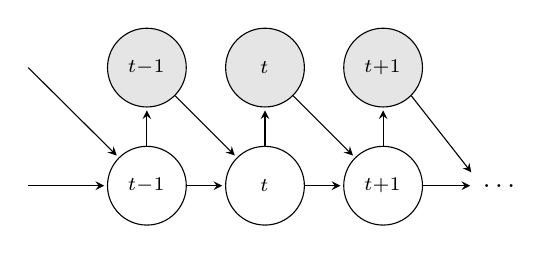
\begin{tikzpicture}[shorten >=1pt]
	\tikzstyle{unit}=[draw,shape=circle,minimum size=1.0cm]
	%\tikzstyle{box}=[draw,shape=rectangle,minimum size=1.0cm,rounded corners]
	
	\node[unit,fill=black!10](xtm1) at (0,1.5){$\vx_{t-1}$};
	\node[unit,fill=black!10](xt) at (1.5,1.5){$\vx_{t}$};
	\node[unit,fill=black!10](xtp1) at (3.0,1.5){$\vx_{t+1}$};
	
	\node[unit,fill=white](htm1) at (0,0){$\vh_{t-1}$};
	\node[unit,fill=white](ht) at (1.5,0){$\vh_{t}$};
	\node[unit,fill=white](htp1) at (3.0,0){$\vh_{t+1}$};
	
	\node (dots) at (4.5,0){\dots};
	
	\draw[-stealth] ([xshift=-1.0cm]xtm1.west) -> (htm1.north west); 
	\draw[-stealth] ([xshift=-1.0cm]htm1.west) -> (htm1.west); 
	
	\draw[-stealth] (htm1.north) -> (xtm1.south); 
	\draw[-stealth] (ht.north) -> (xt.south); 
	\draw[-stealth] (htp1.north) -> (xtp1.south); 
	
	\draw[-stealth] (htm1.east) -> (ht.west); 
	\draw[-stealth] (ht.east) -> (htp1.west); 
	\draw[-stealth] (htp1.east) -> (dots.west); 
	
	\draw[-stealth] (xtm1.south east) -> (ht.north west);
	\draw[-stealth] (xt.south east) -> (htp1.north west);
	\draw[-stealth] (xtp1.south east) -> (dots.north west);
	
\end{tikzpicture}